\section{Clase}
\label{sec:clase}
Hasta ahora se fueron definiendo componentes básicos que pertenecen al estándar
UML, específicamente, subcomponentes los cuales definen, como ya se mencionó,
los datos y el comportamiento de los objetos instanciados, ahora, es necesaria
otra entidad que permita la conjunción de estas herramientas, para eso, se
define el componente de \texttt{clase}.

Recapitulando un poco y volviendo al ejemplo tratado en la \texttt{Sección
\ref{sec:atributo}}, agregando lo que se dijo en el \texttt{Fragmento
\ref{lst:drt_java_modelo_metodo_generico}},
se puede completar la consigna juntando los componentes del lenguaje definidos
y ejemplificados anteriormente junto con el elemento que se está
definiendo aquí en un modelo.

\begin{lstlisting}[caption={Director - Adhiere componente clase al ejemplo},
basicstyle=\footnotesize\ttfamily, label=lst:drt_java_clase]
	class Persona {
		private nombre:string
		private apellido:string
		private DNI:string {@id, @readOnly, @unique}
		public metodo_generico():void
	}
\end{lstlisting}

Lo  cual generaría el siguiente código en un lenguaje como Java:

\begin{lstlisting}[caption={Java - Resultado obtenido de la generación de
\texttt{Fragmento \ref{lst:drt_java_clase}}}, language=Java, basicstyle=\footnotesize\ttfamily]
	class Persona{
		private String nombre;
		private String apellido;
		private String DNI;

		public String get_nombre(){
			return this.nombre;
		}

		public void set_nombre(String nombre){
			this.nombre = nombre;
		}

		public String get_apellido(){
			return this.apellido;
		}

		public void set_apellido(String apellido){
			this.apellido = apellido;
		}

		public String get_DNI(){
			return this.DNI;
		}

		public void set_DNI(String DNI){
			this.DNI = DNI;
		}

		public void metodo_generico() {
			// Implementacion del metodo
		}
	}
\end{lstlisting}


\subsubsection{Analizador Léxico}
El patron que rige el comportamiento de la clase, o al menos el ``esqueleto''
de la misma (esto por el hecho de que se describieron anteriormente los
componentes que van dentro de clases), se describe a continuación:

\begin{lstlisting}
  Regex: class\s*[a-zA-Z0-9_]+\s*\{\s*\}
\end{lstlisting}

Además es posible su representación mediante el siguiente autómata finito:

\begin{figure}[H]
	\centering
	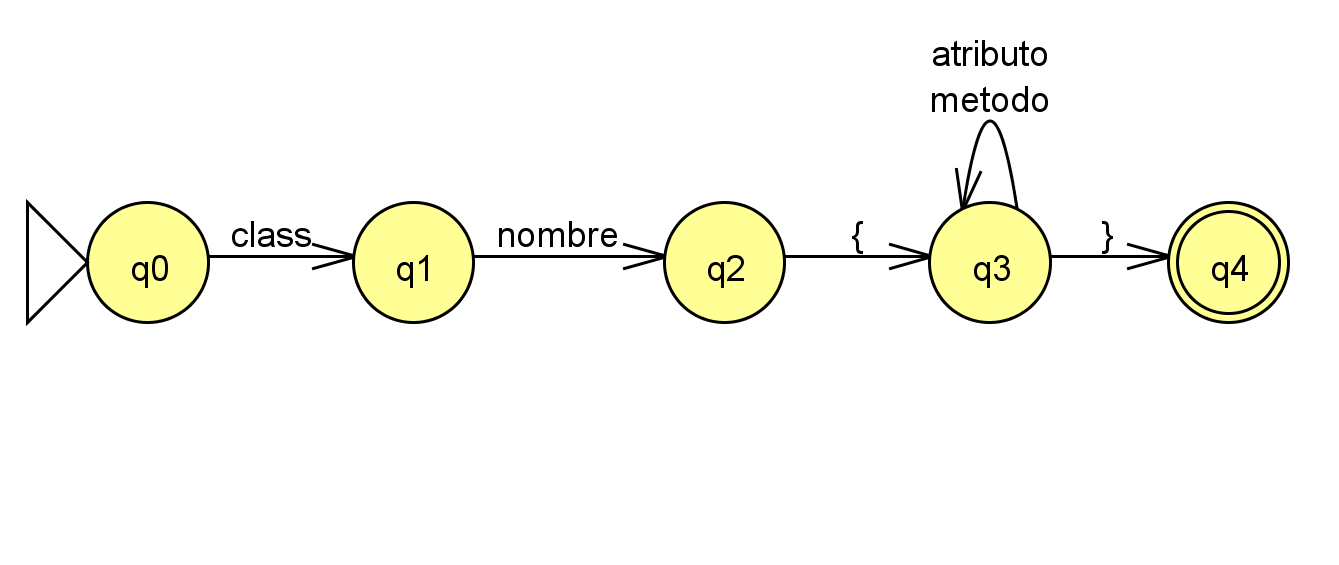
\includegraphics[width=.7\linewidth]{automatas_finitos/classDrt.png}
	\caption{Autómata finito - Clase}
	\label{fig:af_clase}
\end{figure}

\subsubsection{Analizador Sintáctico}
La notación BNF para la definición de una clase en Director es la siguiente:

\begin{lstlisting}[caption={BNF - Clase}, basicstyle=\footnotesize\ttfamily]
  <clase> ::= "class" <nombre> "{" <atributos> | <metodos> "}"
\end{lstlisting}

Los subcomponentes se trataron en secciones anteriores del documento, de todas
formas se detalla el BNF correspondiente a la pluralización de los mismos.

\begin{lstlisting}[basicstyle=\footnotesize\ttfamily]
  <atributos> ::= <atributo> | <atributos>
\end{lstlisting}

\begin{lstlisting}[basicstyle=\footnotesize\ttfamily]
  <metodos> ::= <metodo> | <metodos>
\end{lstlisting}


\subsubsection{Derivaciones Clase}

Nuevamente ya se cuentan con los  patrones y las representaciones visuales
que rigen
el uso del componente, ahora se procede a estudiar los pasos a seguir en cuanto al
análisis sintáctico, aquí se veran las derivaciones que siguen de un ejemplo,
junto con el árbol sintáctico del mismo.

El ejemplo a tomarse para el análisis se describe a continuación:

\begin{lstlisting}
EJEMPLO: class Persona{\n
            - DNI:integer\n
            - nombre:string\n
            + toString():void\n
          }
\end{lstlisting}

Por cuestiones de espacio y de lo extenso de las derivaciones para los
componentes, se tomaron abreviaciones para los componentes, a continuación
se detalla el significado de cada una de ellos.

\begin{itemize}
  \item \textbf{PR}: palabra reservada
  \item \textbf{V}: visibilidad
  \item \textbf{N}: nombre
  \item \textbf{SE}: simbolo especial
  \item \textbf{T}: tipo
  \item \textbf{A}: atributo
  \item \textbf{M}: metodo
\end{itemize}

\begin{lstlisting}[basicstyle=\ttfamily\footnotesize]
  comp-drt -> clase
  clase -> PR N SE A A M SE
  clase -> class N SE A A M SE      <- luego de ese punto se deben
  clase -> class Persona SE A A M SE   extender los atributos y el
  clase -> class Persona{ A A M SE      metodo
  clase -> class Persona{atr:DNI A M SE
  clase -> class Persona{atr:DNI A M SE
  clase -> class Persona{DNI:integer \n nombre \n toString():string}
\end{lstlisting}

Si bien en el ejemplo se tienen atributos y un método, estos no se expanden de
manera adecuada en las derivaciones, esto se debe al espacio que se terminaria
teniendo, las derivaciones que se tienen que realizar son exactamente como las
que ya se tuvieron en las secciones anteriores.

